\subsection{Flutter}
\label{sec:frameworks_flutter}

Das Framework Flutter wird primär von Google entwickelt und wurde 2018 in Form der ersten Beta-Version veröffentlicht \cite{Sharma_Flutter}.
Flutter setzt einen starken Fokus auf \ac{UI} mobiler Anwendungen und zielt darauf ab, die Benutzerschnittstellen an den Stil der jeweiligen Plattform anzupassen \cite{Flutter_Architektur}.


Die Basis von Flutter bildet die, ebenfalls von Google entwickelte, Programmiersprache Dart.
Dart ist darauf ausgelegt, eine Vielzahl von Plattformen, darunter Android, iOS und Webanwendungen, direkt zu unterstützen.
Dazu unterstützt Dart die Kompilierung in nativ ausführbaren Code mittels eines \ac{AOT}-Compilers, während für Webanwendungen eine Transpilation in JavaScript erfolgt \cite{Flutter_Architektur,Dart_Overview}.


Flutter verwendet für die Unterstützung der mobilen Plattformen eine dreischichtige Architektur.
Wie in \autoref{fig:flutter_architecture} gezeigt, besteht diese aus den Schichten \textit{Framework}, \textit{Engine} und \textit{Embedder}.
Die eigentliche Anwendung wird oberhalb der Framework-Schicht umgesetzt und kann die Abstraktionen verwenden, die von den darunterliegenden Schichten bereitgestellt werden.
\begin{figure}[h]
    \centering
    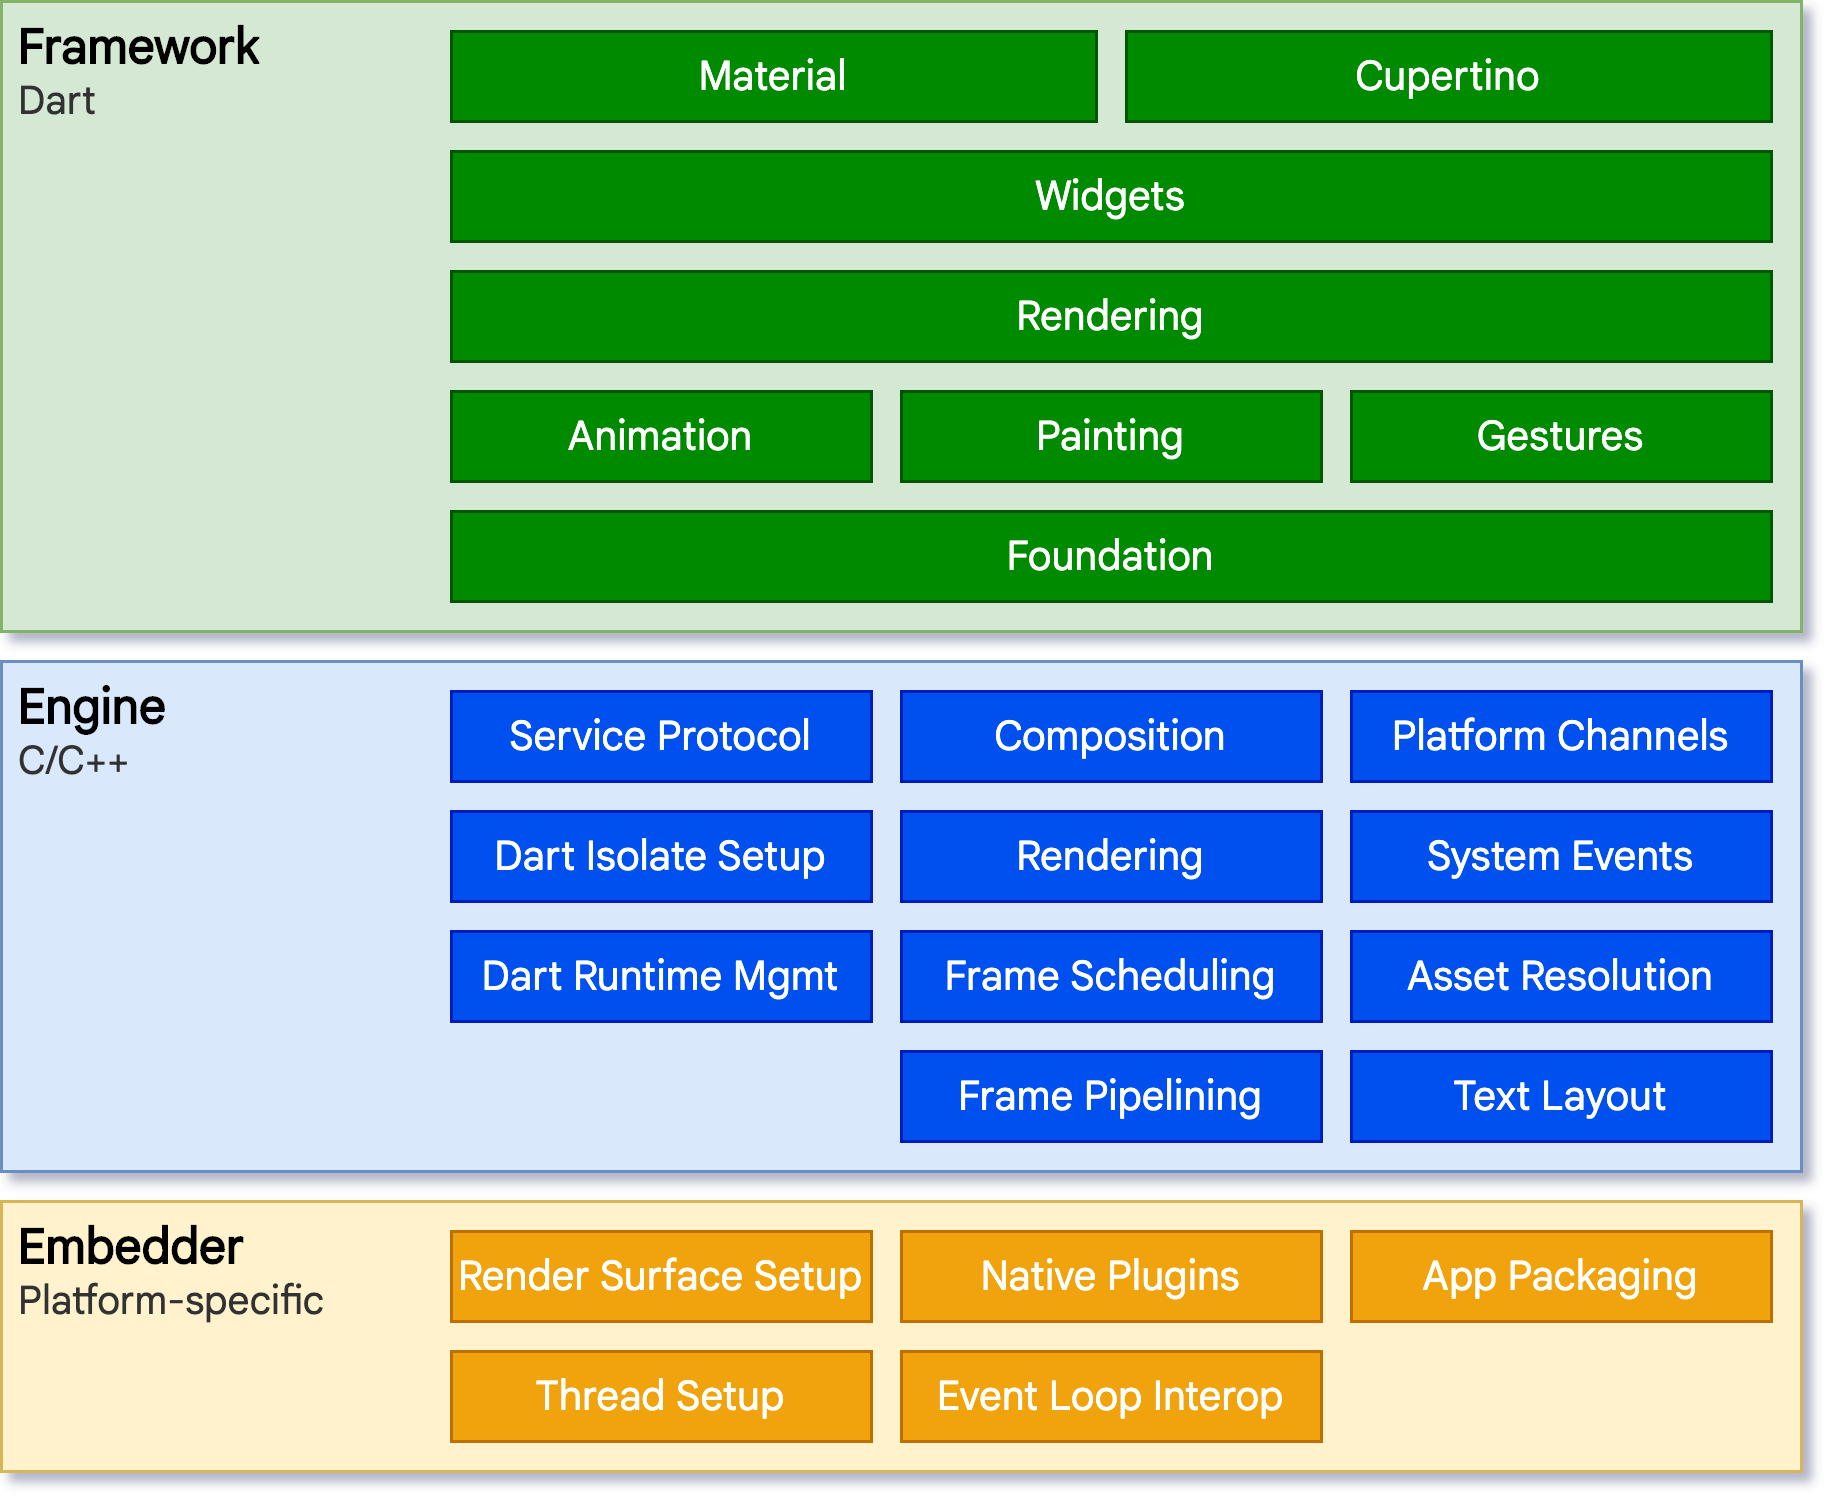
\includegraphics[height=10cm]{flutter_architecture.png}
    \caption{Schichtenarchitektur des Flutter-Frameworks \cite{Flutter_Architektur}}
    \label{fig:flutter_architecture}
\end{figure}


Die Basis bildet die Embedder-Schicht, welche als einzige plattformspezifisch ist und den darüber liegenden Schichten eine einheitliche Schnittstelle zum unterlagerten System zur Verfügung stellt.
Für die verbreiteten Plattformen, wie Android und iOS, steht eine Standard-Implementierung bereit.
Zusätzlich können jedoch auch eigene Embedder implementiert werden, um weitere Plattformen zu unterstützen \cite{Flutter_Architektur}.


Auf den Embedder setzt die Flutter-Engine auf, welche die Flutter-\acp{API} bereitstellt, und das Rendering der Oberfläche übernimmt.
Anstatt auf die \ac{UI}-Bibliotheken des unterlagerten Systems zurückzugreifen, verwendet Flutter die \textit{Skia Graphics Engine} um Steuerelemente zu rendern \cite{Biorn-Hansen_PerformanceOverhead_CrossPlatform}.
Skia ist für alle gängigen Plattformen verfügbar und wird mit jeder Flutter-Anwendung ausgeliefert.
Das Flutter-Team gibt an, dass durch den Verzicht auf die Verwendung systemeigener Bibliotheken eine Abstraktionsebene eingespart werden kann, was zu hoher Performance beim \ac{UI}-Rendering führt \cite{Flutter_Architektur}.


Die Framework-Schicht abstrahiert den Zugriff, sodass Funktionen der unterlagerten Schichten in der Programmiersprache Dart verwendet werden können.
Außerdem finden sich auf dieser Ebene verschiedene optional eingebundene Bibliotheken des Frameworks.
Zum Erhalt der \ac{UI}-Konsistenz werden zum Beispiel die beiden Bibliotheken Material und Cupertino eingesetzt, welche für Steuerelementen den Stil von Google respektive Apple nachahmen können \cite{Manchanda_CrossPlatformFrameworks, Flutter_Architektur}.


Durch die Abstraktionen des Frameworks sind einige native Funktionen direkt oder über offizielle Bibliotheken verfügbar \cite{Dart_Overview}.
Darüber hinaus bietet Flutter auch die Möglichkeit, beliebigen Code in der nativen Sprache der jeweiligen Plattform aufzurufen.
Damit lassen sich alle \acp{API} der Betriebssysteme nutzen.
Für häufig eingesetzte Funktionen stehen hierfür Open-Source Plugins bereit, sodass nicht jede Funktionalität neu entwickelt werden muss \cite{Flutter_Architektur}.
Werden spezielle Funktionen benötigt, müssen jedoch eigene Plugins entwickelt werden.


Zur allgemeinen Bewertung der Performance von Flutter existieren widersprüchliche Aussagen.
So gibt es Situationen, in denen Flutter die Performance einer nativen Anwendung sogar übertrifft und ansonsten meist besser abschneidet als Implementierungen mit anderen Frameworks \cite{Nawrocki_Comparison_Hybrid_Native_Frameworks}.
Allerdings zeigen Bi{\o}rn-Hansen \textit{et al.} \cite{Biorn-Hansen_PerformanceOverhead_CrossPlatform}, dass die mittlere Zeit zur Ausführung einer definierten Aufgabe bei mit Flutter entwickelten Apps deutlich höher ist als bei äquivalenten Apps, die mit anderen Technologien entwickelt wurden.

Es ist davon auszugehen, dass diese Widersprüche auf verschiedene Anwendungsfälle und unterschiedliche Testmethodiken zurückzuführen sind.
Dementsprechend ist die Performance von Flutter vom konkreten Einsatzzweck und der Zielplattform abhängig.
Weiterhin liefern die genannten Untersuchungen keine Aussagen zur Performance im Anwendungsfall einer Videoaufzeichnung.

Nur vier Jahre nach dem Release der ersten Beta-Version \cite{Sharma_Flutter} ist Flutter in der Stack Overflow Umfrage 2022 \cite{Stackoverflow_2022}, das unter Entwicklern beliebteste Cross-Plattform Framework.
Eine Mehrheit von 68,03 \% der befragten Entwickler, welche bereits mit Flutter gearbeitet haben, gibt an, das Framework auch in Zukunft einsetzen zu wollen.
Weiterhin wollen 13,52 \% aller Entwickler ohne Erfahrung mit dem Framework, zukünftig mit Flutter arbeiten, was ebenfalls von keinem anderen Cross-Plattform Framework übertroffen wird.

